\begin{figure}[!ht]
\centering
\caption{Robô após montagem}
\label{fig:RoboReal2}
	\begin{subfigure}[b]{0.49\textwidth}%
		\centering
		% fbox{}
		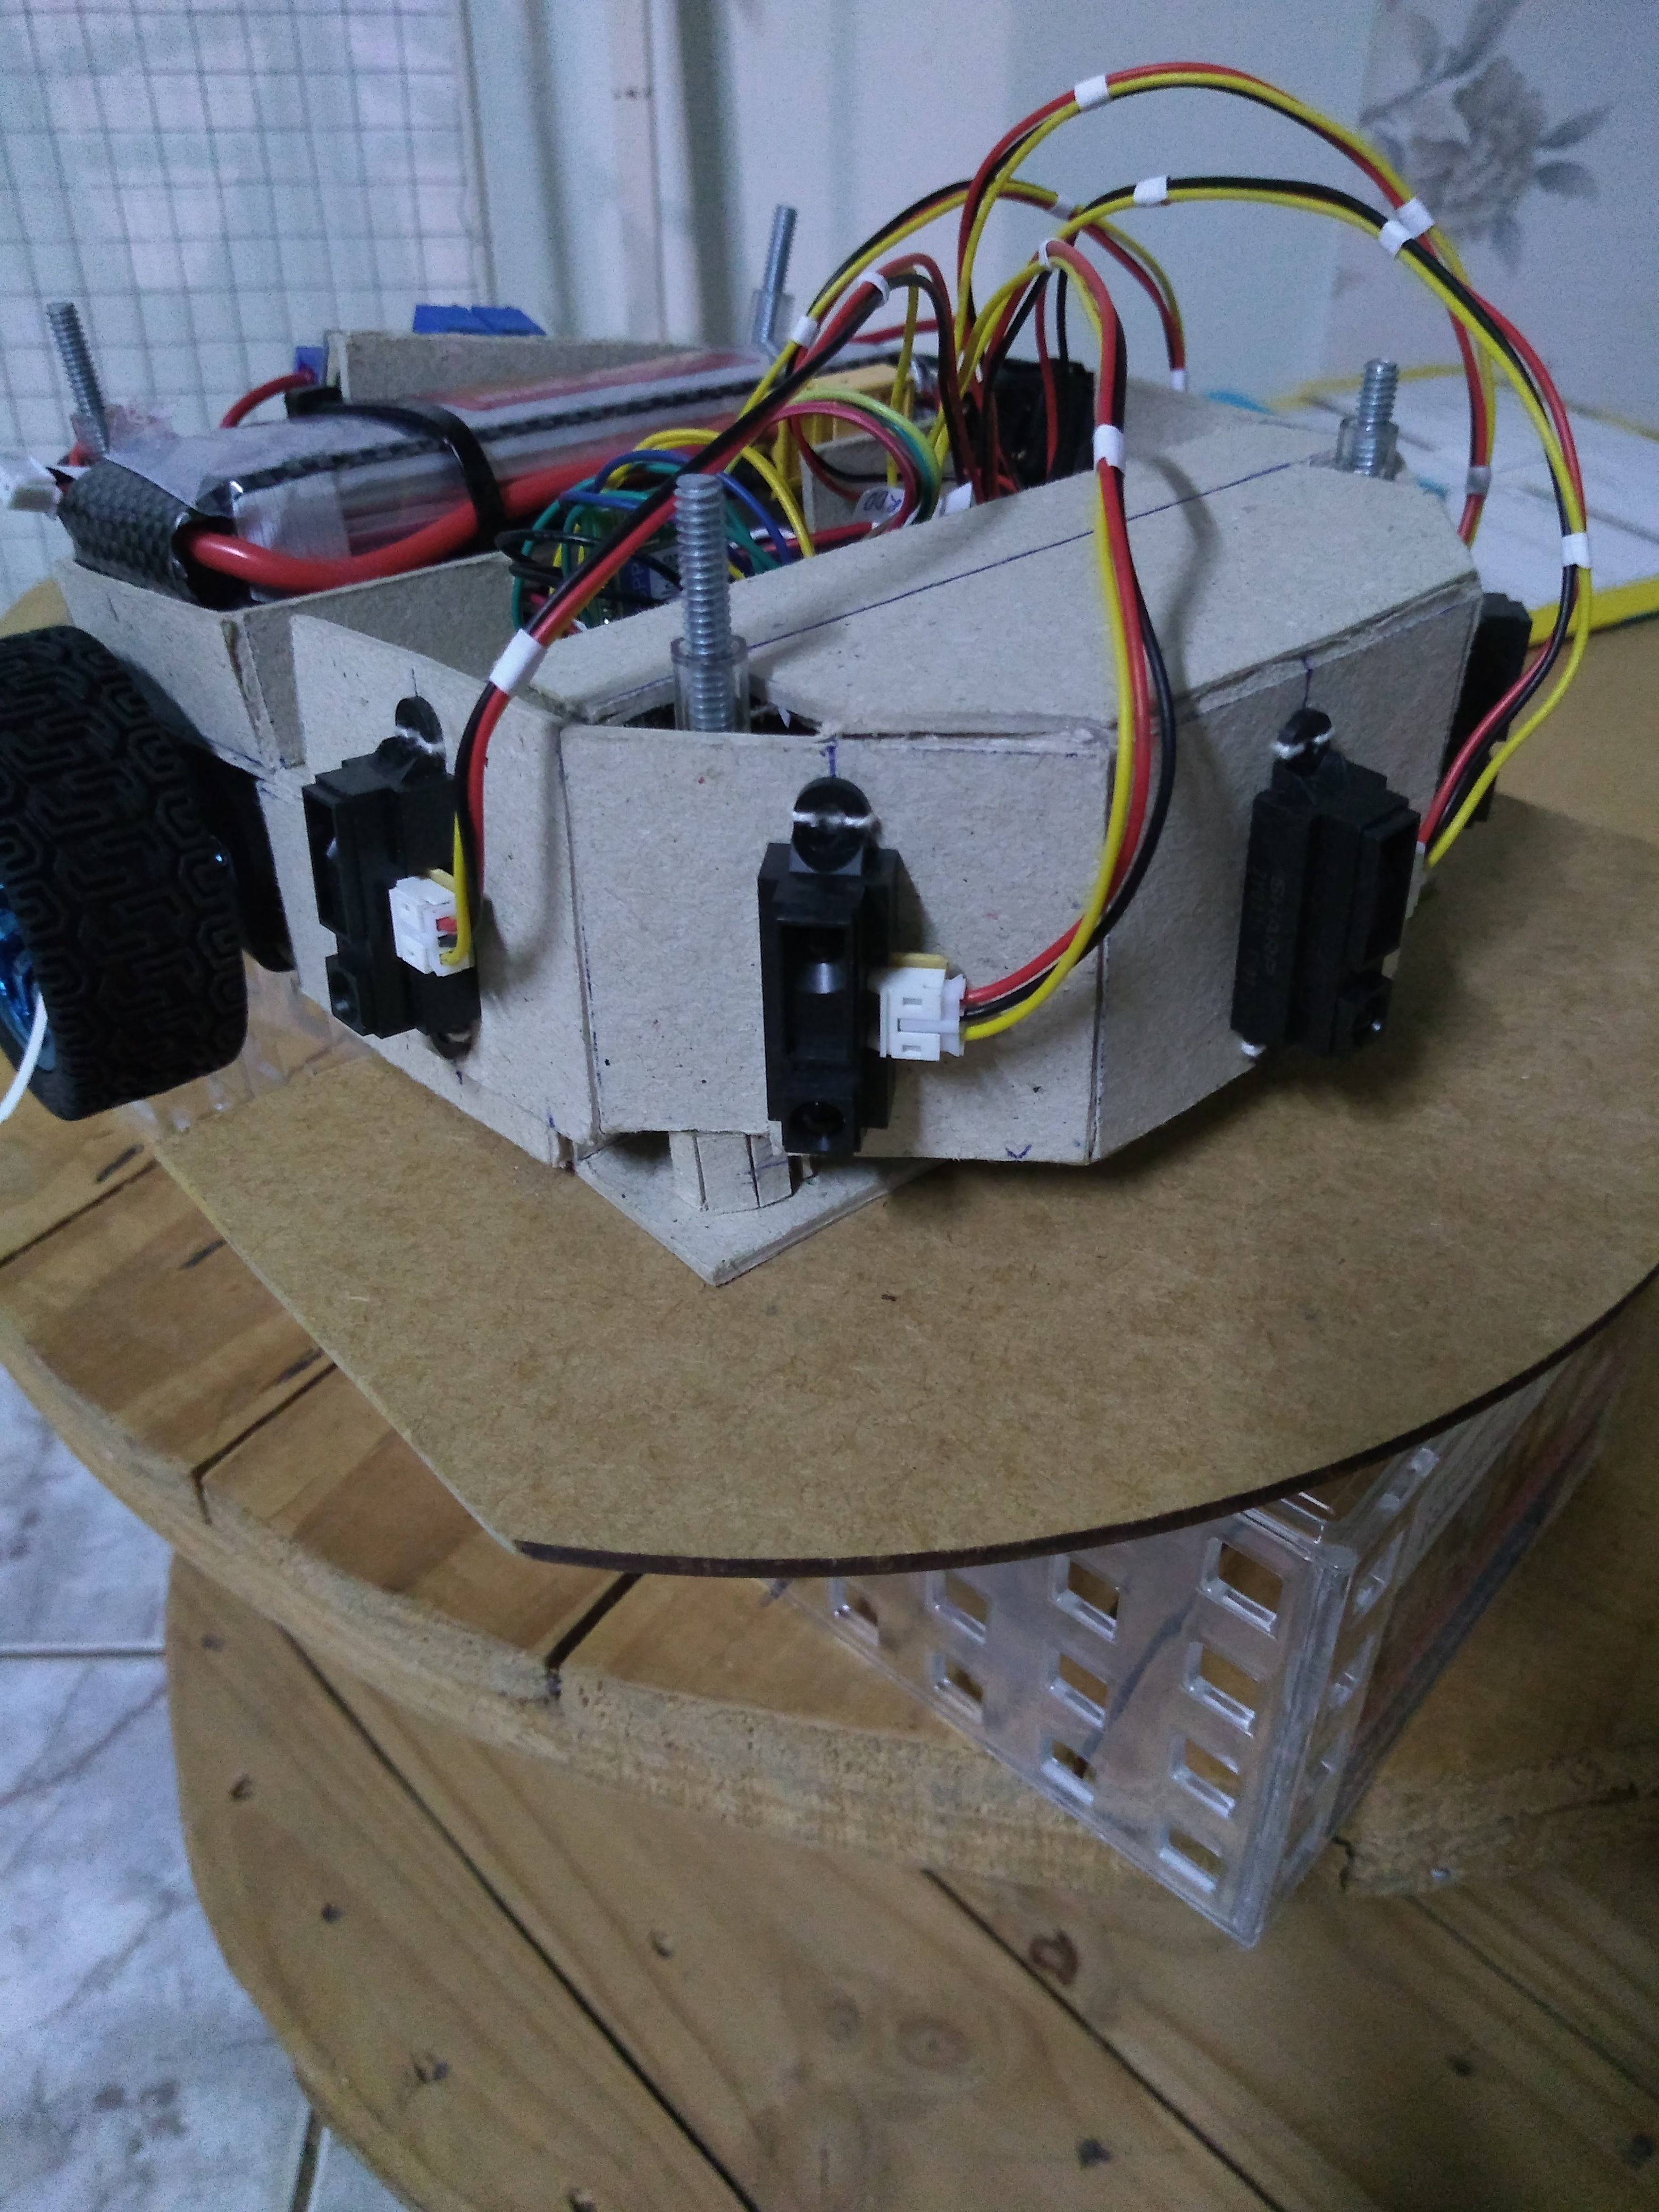
\includegraphics[trim={0cm 35cm 0cm 0cm}, clip, 
		scale=0.055]{Figuras/RoboMontagem5}
		\subcaption{Posição dos parafusos de rosca}
	  	%\label{fig:test1}
	\end{subfigure}
	~
	\begin{subfigure}[b]{0.49\textwidth}%
		\centering
		% fbox{}
		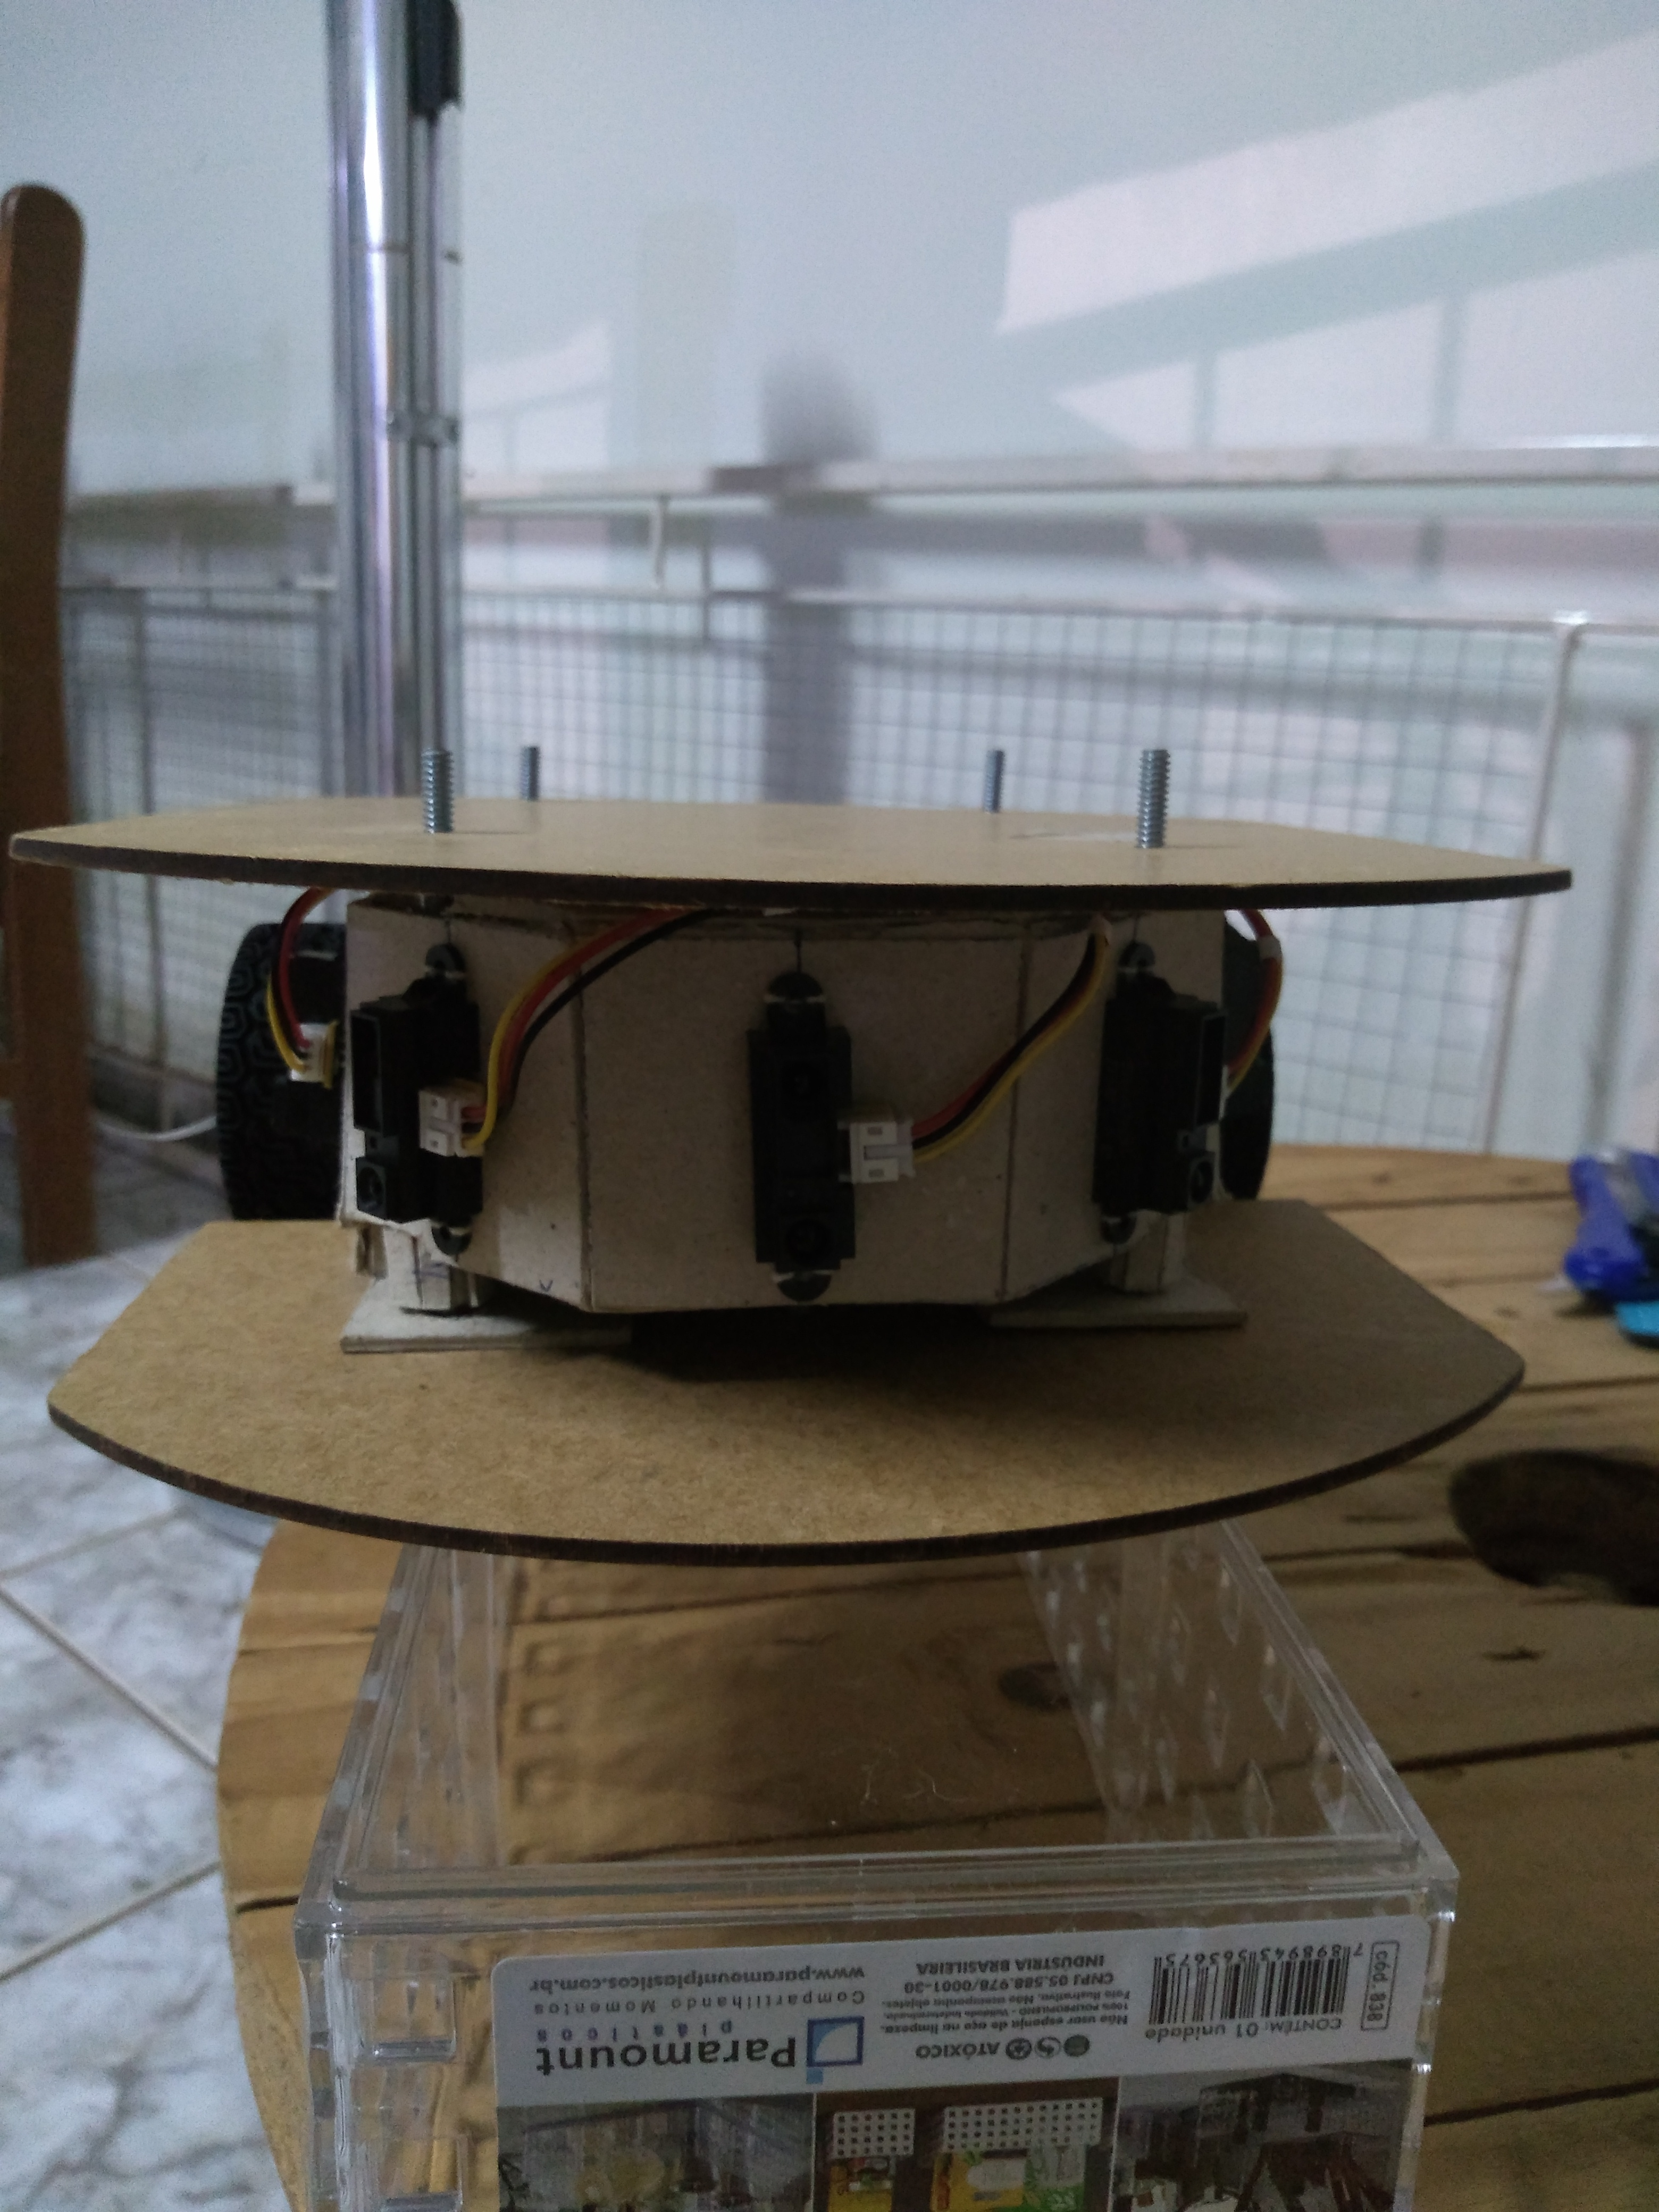
\includegraphics[trim={0cm 12.5cm 0cm 22.5cm}, clip, 
		scale=0.055]{Figuras/RoboMontagem6}
		\subcaption{Robô montado}
	  	%\label{fig:test2}
	\end{subfigure}
	\textbf{Fonte: autoria própria}
\end{figure}